% LaTeX template adapted from: https://www.overleaf.com/latex/templates/simple-math-homework-template/tbszsswsndrz
\documentclass[landscape,10pt]{article}
\usepackage[utf8]{inputenc}
\usepackage[english]{babel}
\usepackage[]{amsthm} %lets us use \begin{proof}
\usepackage[]{amssymb} %gives us the character \varnothing
\usepackage{amsmath} %for equations
\usepackage[]{listings} %for code blocks
\usepackage{graphicx} %for diagrams
\usepackage{fancyhdr} %for headers
\usepackage[letterpaper, margin=0.5in]{geometry}
\usepackage{tikz} % for drawings
\usepackage{multicol}
\usepackage{ifthen}
\usepackage{enumitem}
\setlist{nolistsep}
\setlist[itemize]{leftmargin=0.5pc,itemsep=0.25em}
\usetikzlibrary{arrows.meta,shapes.arrows,chains,decorations.pathreplacing}
\makeatletter
\renewcommand{\section}{\@startsection{section}{1}{0mm}%
            {-1ex plus -.5ex minus -.2ex}%
            {0.5ex plus .2ex}%x
            {\normalfont\large\bfseries}}
\renewcommand{\subsection}{\@startsection{subsection}{2}{0mm}%
            {-1explus -.5ex minus -.2ex}%
            {0.5ex plus .2ex}%
            {\normalfont\normalsize\bfseries}}
\renewcommand{\subsubsection}{\@startsection{subsubsection}{3}{0mm}%
            {-1ex plus -.5ex minus -.2ex}%
            {1ex plus .2ex}%
            {\normalfont\small\bfseries}}
\makeatother

\newcommand{\code}[1]{\texttt{#1}}

\pagestyle{empty}
\ifthenelse{\lengthtest { \paperwidth = 11in}}
{ \geometry{top=.5in,left=.5in,right=.5in,bottom=.5in} }
{\ifthenelse{ \lengthtest{ \paperwidth = 297mm}}
{\geometry{top=1cm,left=1cm,right=1cm,bottom=1cm} }
{\geometry{top=1cm,left=1cm,right=1cm,bottom=1cm} }
}
\setlength{\parindent}{0em}
\setlength{\parskip}{-0.25em}

\graphicspath{ {./}}

\begin{document}
\footnotesize
\begin{multicols}{4}
\setlength{\premulticols}{1pt}
\setlength{\postmulticols}{1pt}
\setlength{\multicolsep}{1pt}
\setlength{\columnsep}{2pt}
\subsubsection*{Some Formulae:}
\begin{itemize}
    \item[] \(\text{Power} = \text{Capacity} \cdot \text{Voltage}^2 \cdot \text{Frequency}_{0 \rightarrow 1} + \text{Voltage}\cdot I_{\text{leakage}}\)
    \item[] \(\text{Power} = \frac{\text{Joules}}{\text{Op}} \cdot \frac{\text{Ops}}{\text{Second}}\)
    \item[] Dennard scaling: 0.7x voltage drop 
    \item[] Latency: How long it takes to do a task
    \item[] Throughput: Total work done per unit of time e.g. queries/sec
    \item[] Clock period: Duration of a clock cycle
    \item[] Clock frequency: cycles per second
    \item[] Response time \(T = T_0 \frac{\rho}{1-\rho}\) with \(\rho = \) percentage of throughput
    \item[] \(\text{Execution Time} = \text{Cycles per Program} \cdot \text{Clock Cycle Time} = \frac{\text{Cycles Per Program}}{\text{Clock Rate}}\)
    \item[] \(\text{Clock Cycles} = \text{Instruction Count} \cdot \text{Cycles per Instruction}\)
    \item[] \(\text{CPU Time} = \text{Instruction Count} \cdot \text{CPI} \cdot \text{Clock Cycle Time} = \frac{IC \cdot CPI}{\text{Clock Rate}}\)
    \item[] \(\text{Exec Time} = \frac{\text{Instructions}}{\text{Program}} \cdot \frac{\text{Clock Cycles}}{\text{Instruction}} \cdot \frac{\text{Seconds}}{\text{Clock Cycle}}\)
    \item[] Clock Cycles \(= \sum \limits_{i = 1}^{n} \big ( CPI_i \cdot IC_i \big) \)
    \item[] Weighted average CPI \(= \frac{\text{Clock Cycles}}{\text{Instruction Count}} = \sum \limits_{i=1}^{n} \Big ( CPI_i \cdot \frac {IC_i}{IC} \Big ) \)
    \item[] Performance \(= \frac{1}{\text{Exec Time}}\)
    \item[] ``\(X\) is \(n\) faster than \(Y\)'' means \(\frac{Perf_X}{Perf_Y} = \frac{Exec_Y}{Exec_X} = n\)
    \item[] Energy = Average Power x Execution Time
    \item[] Optimize for Energy per Instruction: \(Power = \frac{energy}{second} = \frac{energy}{instruction} \cdot \frac{instructions}{second}\)
    \item[] Amdahl's Law: \(Speedup = \frac{CPUTime_{old}}{CPUTime_{new}} = \frac{CPUTime_{old}}{CPUTime_{old} [(1 - f_x) + \tfrac{f_x}{S_x}]} = \frac{1}{(1 - f_x) + \tfrac{f_x}{s_x}}\)
    \item[] Parallel Speedup: \(Speedup = \frac{1}{(1 - P) + \tfrac{P}{n}} \rightarrow P = \frac{\frac{1}{Speedup} - 1}{\tfrac{1}{n} - 1}\)
    \item[] Arithmetic Mean: \(\frac{1}{n} \sum \limits_{i=1}^{n}T_i\) used with times, not rates
    \item[] Harmonic mean: \(\frac{n}{\sum \limits_{i=1}^{n}\frac{1}{R_i}}\) used with rates not times
    \item[] Geometric mean: \(\Bigg ( \prod \limits_{i=1}^{n} \frac{T_i}{T_{ri}} \Bigg)^{\tfrac{1}{n}} = \exp\Bigg(\frac{1}{n}\sum \limits_{i=1}^{n}\log\Big(\frac{T_i}{T_{ri}}\Big) \Bigg)\)
    \item[] Power/performance benchmark: Overall ssj\_ops per Watt = \(\frac{\Big(\sum \limits_{i=0}^{10}ssj\_ops_i\Big)}{\Big(\sum\limits_{i=0}^{10}Power_i\Big)}\)
    \item[] Perf metrics: 
    \begin{itemize}
        \item[] \code{time <application>} measures execution time
        \item[] \code{perf record} does low overhead sampling
        \item[] \code{perf topdown} uses hardware performance counters
    \end{itemize}
    \item[] Flip flop setup time: \(t_{ck} > t_{pd} + t_s + t_{skew}\)
\end{itemize}

\subsubsection*{CISC:} Multi-cycle complex instructions; Load/store incorporated in instruction; Small code size; High CPI; Low clock frequency; Variable length instructions

\subsubsection*{RISC:} Simple (single-clock) Instructions; Register-to-register separate load instructions; Large code size; Low CPI; High clock frequency; Same length instructions; Simple instruction decode; 
\subsubsection*{Call and Return:}
\begin{itemize}
    \item[] Caller:
    \begin{itemize}
        \item[] Save caller-saved registers as needed
        \item[] Load arguments
        \item[] Execute \code{JAL}
    \end{itemize}
    \item[] Callee setup:
    \begin{itemize}
        \item[] Allocate memory for new frame (\code{xsp} = \code{xsp} - frame)
        \item[] Save callee-saved registers as needed
        \item[] Set frame pointer (\code{xfp} = \code{xsp} + frame size - 4)
    \end{itemize}
    \item[] Callee return:
    \begin{itemize}
        \item[] Place return values in \code{x10} and \code{x11}
        \item[] Restore any callee-saved registers
        \item[] Pop stack (\code{xsp} = \code{xsp} + frame size)
        \item[] Return by \code{jr xra}
    \end{itemize}
    \item[] Caller:
    \begin{itemize}
        \item[] Restore any caller-saved registers as needed
    \end{itemize}
\end{itemize}
\subsubsection*{Pipeline stages:}
\begin{itemize}
    \item[] \code{IF}: Instruction fetch
    \item[] \code{ID}: Instruction decode, register read
    \item[] \code{EX}: execute operation or calculate address
    \item[] \code{MEM}: Access memory command
    \item[] \code{WB}: Write result back to register
\end{itemize}
\subsubsection*{Hazards:}
\begin{itemize}
    \item[] Structure Hazards: A required hardware resource is busy
    \item[] Data hazards: Must wait for previous instructions to produce/consume data
    \begin{itemize}
        \item[] Read after Write: Instruction \(j\) tries to read before instruction \(i\) tries to write it
        \item[] Write after Write: Instruction \(j\) tries to write an operand before \(i\) writes its value
        \item[] Write after Read: Instruction \(j\) tries to write a destination before it is read by \(i\)
    \end{itemize}
    \item[] Control hazards: Next \code{PC} depends on current instruction result
\end{itemize}
\subsubsection*{Forwarding:}
\begin{itemize}
    \item[] Identify \textit{producers}: \code{EX} and \code{MEM} stages
    \item[] All stages after first producer are sources of forwarding data: \code{MEM} and \code{WB}
    \item[] Identify \textit{consumers}: \code{EX} and \code{MEM}
    \item[] These are the destinations of forwarded data
\end{itemize}
\subsubsection*{Branch Prediction:}
\begin{itemize}
    \item[] Static: predict not-taken
    \item[] Dynamic:
    \begin{itemize}
        \item[] Branch History Table: one entry for each branch, taken/not taken record
        \item[] Branch Target Buffer: One entry for each branch, computes target address
    \end{itemize}
\end{itemize}
\subsubsection*{Exceptions and Interrupts:}
\begin{itemize}
    \item[] Switch from `user' to `kernel' mode
    \item[] Exceptions: Arises within CPU. Undefined opcode, overflow, etc
    \item[] Interrupt: External I/O controller, network card, etc
    \item[] On exceptions:
    \begin{itemize}
        \item[] Pass to relevant handler
        \item[] Then return to program using EPC if possible
        \item[] All previous instructions completed
        \item[] Faulting instruction not started
        \item[] No side effects
    \end{itemize}
    \item[] Nullifying instructions: Converts them to a NOP
\end{itemize}
\subsubsection*{Going past the 5-stage pipeline:}
\begin{itemize}
    \item[] Instruction-level Parallelism: Independence among instructions; Fetch multiple instructions per cycle; Evaluate which ones can go down the pipe together
    \item[] Superscalar: Double up on hardware in order to execute multiple instructions simultaneously
    \item[] Deeper Pipelines: Increase the number of stages, decrease amount of logic. Higher clock freq.
    \item[] Register Renaming: Map architectural registers to physical registers in decode stage to get rid of false dependencies. Need more physical registers than architectural ones.
    \item[] Data flow graph:
    \begin{itemize}
        \item[] Scoreboard: bit array, 1-bit for each GPR
        \begin{itemize}
            \item[] If the bit is not set, the reg has valid data
            \item[] If the bit is set, the reg has stale data
        \end{itemize}
        \item[] Dispatch in order: RD \(\leftarrow\) Fn(RS,RT)
        \begin{itemize}
            \item[] If \code{SB[RS]} or \code{SB[RT]} is set \(\rightarrow\) RAW, stall
            \item[] If \code{SB[RD]} is set \(\rightarrow\) WAW, stall
            \item[] Else dispatch to functional unit, set \code{SB[RD]}
        \end{itemize}
        \item[] Complete out-of-order
        \item[] Update \code{GPR[RD]}, clear \code{SB[RD]}
    \end{itemize}
\end{itemize}

\subsubsection*{Caching:}
\begin{itemize}
    \item[] AMAT: \(\text{Access Time} = \text{hit time} + \text{miss rate} \cdot \text{miss penalty}\)
    \item[] Three C's of misses:
    \begin{itemize}
        \item[] Compulsory: First time you've accessed this item
        \item[] Capacity: Not enough room in the cache to hold item
        \item[] Conflict: Item was replaced because of a conflict in its set
    \end{itemize}
    \item[] Direct-mapped cache:
    \begin{itemize}
        \item[] \(2^n\) bytes total with \(2^m\) byte blocks
        \item[] Byte select: lower \(m\) bits
        \item[] Cache index: lower \((n-m)\) bits of the memory address
        \item[] Cache tag: upper \(32-n\) bits of the memory address
    \end{itemize}
    \item[] \(N\)-way set associative:
    \begin{itemize}
        \item[] Each memory block can go to one of \(N\) entries in the cache
        \item[] \(2^n\)-byte cache, \(2^m\)-byte blocks, \(2^a\) set-associative:
        \begin{itemize}
            \item[] Cache contains \(2^n/2^m = 2^{n-m}\) blocks
            \item[] Each cache way contains \(2^{n-m}/2^a = 2^{n-m-a}\) blocks
            \item[] Byte offset: lowest \(m\) bits
            \item[] Cache index: next \(n-a\) bits
        \end{itemize}
        \item[] Associative caches might use Least Recently Used table for evictions
        \item[] For \(N\)-way cache, \(N!\) orderings
    \end{itemize}
    \item[] Write-through:
    \begin{itemize}
        \item[] Main memory updated each cache write
        \item[] Replacing a cache entry just overwrites new block
        \item[] Memory write may cause pipeline stalls
        \item[] Misses are simpler and cheaper
        \item[] Uses a write buffer | FIFO queue
    \end{itemize}
    \item[] Write-back:
    \begin{itemize}
        \item[] Only the cache entry is updated on each cache write
        \item[] Cache and memory entries are inconsistent
        \item[] Add `dirty' bit to indicate whether memory needs to be updated
        \item[] Write new value to memory on evictions
        \item[] Writes are super fast
    \end{itemize}
    \item[] Write miss options: Do you allocate for space in the cache on a miss?
    \item[] Do you fetch the rest of the block contents from memory?
    \item[] For no-fetch-on-miss must use fine-grained valid bits
    \item[] Write-back: typically write-allocate, fetch-on-miss
    \item[] Multilevel caches:
    \begin{itemize}
        \item[] Primary L1 caches attached to CPU: small, fast, focuses on hit time
        \item[] Secondary L2 caches service misses from L1: larger, slower, still faster than DRAM
    \end{itemize}
    \item[] Cache Coherency:
    \begin{itemize}
        \item[] \(P\) writes \(X\), \(P\) reads \(X \rightarrow \) read returns written value
        \item[] \(P_1\) writes \(X\), \(P_2\) reads \(X\) later \(\rightarrow \) read returns written value
        \item[] \(P_1\) writes \(X\), \(P_2\) writes \(X \rightarrow\) all processors see writes in the same order
        \item[] Single-Writer, Multiple-Read Invariant: For any memory location \(A\), at any given epoch, there exists only one CPU that may write to \(A\) or some number of CPUs that may only read \(A\)
        \item[] Data-Value Invariant: The value of the memory location at the start of an epoch is the same as the value of the memory location at the end of its last read-write epoch
        \item[] CPU uses snooping protocols to ensure this:
        \begin{itemize}
            \item[] 2-state: very simple hardware and protocol. Write-through, all writes go on interconnect bus.
            \item[] 3-state MSI: Modified (one cache has valid copy), Shared (one or more have read-only copy), Invalid (invalidated so one copy can go to modify state)
        \end{itemize}

    \end{itemize}
\end{itemize}

\subsubsection*{DRAM:} SRAM is 6 transistors, static, doesn't need refresh, used for caches. DRAM is 1 transistor + 1 capacitor, needs refresh every ~10ms, much higher capacity. DRAM outputs data in bursts (I guess x8 at a time?). DRAM accesses:
\begin{itemize}
    \item[] \code{ACTIVATE} to open a row
    \item[] \code{READ} to read a column
    \item[] \code{WRITE} to write to a column
    \item[] \code{PRECHARGE} to close a row
    \item[] \code{REFRESH} on timed interval
\end{itemize}
In order to access a `closed' row, must first \code{PRECHARGE} the row that is open, then \code{ACTIVATE} the row to be read, then \code{READ/WRITE} to access row buffer. Modern DRAM has BANKS which operate independently of each other but use the same access hardware. Each bank can have a different row active. The \code{ACTIVATE} and \code{PRECHARGE} latencies can overlap. Physical constraints:
\begin{itemize}
    \item[] \code{tRCD} = Row to Column command delay (how long it takes row to get to sense amp)
    \item[] \code{tCAS} = Time between column command and data out
    \item[] \code{tCCD} = time between column commands (rate that these can be pipelined)
    \item[] \code{tRP} = time to precharge DRAM array
    \item[] \code{tRAS} = time between row activation and data restoration (minimum time row must be open)
    \item[] \code{tRC = tRAS + tRP} = row `cycle' time
\end{itemize}
Timing constraints:
\begin{itemize}
    \item[] CPU \(\rightarrow\) memory controller transfer time
    \item[] controller latency
    \item[] DRAM bank latency:
    \begin{itemize}
        \item[] \code{tCAS} if row is open
        \item[] \code{tRCD + tCAS} if array is precharged
        \item[] \code{tRP + tRCD + tCAS} worst case
    \end{itemize}
    \item[] DRAM transfer time = BurstLen/(MT/s)
    \item[] Memory controller \(\rightarrow\) CPU transfer time
\end{itemize}

\subsubsection*{Virtual Memory:} OS maps virtual addresses to physical memory using a page table. One page table per process. If a page isn't mapped it generates a page fault, which traps to OS, to map a new page. Translation Lookaside Buffer \code{TLB} is a hardware cache for page tables. Each \code{TLB} entry stores a page table entry \code{PTE}. \code{TLB} is like a cache and uses tag, valid, dirty bits. Page size depends on application, OS and kernel use large pages but user applications frequently use smaller. Page table size is \code{(num pages) * (page entry width)}. Hierarchical page tables: First level stores directory, second level stores actual page entries. Only top level needs to be resident in memory. Abbreviations:
\begin{itemize}
    \item[] \code{MMU}: Memory Management Unit controls \code{TLB}
    \item[] Components of the virtual address \code{VA}:
    \begin{itemize}
        \item[] \code{TLBI}: TLB index
        \item[] \code{TLBT}: TLB tag
        \item[] \code{VPO}: Virtual page offset
        \item[] \code{VPN}: virtual page number
    \end{itemize}
    \item[] Components of the physical address \code{PA}:
    \begin{itemize}
        \item[] \code{PPO}: phys. page offset
        \item[] \code{PPN}: phys. page number
        \item[] \code{CO}: byte offset within cache line
        \item[] \code{CI}: cache index
        \item[] \code{CT}: cache tag
    \end{itemize}
\end{itemize}
\subsubsection*{VIPT:} \code{VIPT} uses virtual address bits for indexing and physical address bits for tag. The cache uses the physical address as the tag. The \code{TLB} uses the virtual address as the index and has the tag stored as its data. An access means indexing in the \code{TLB}, getting the \code{TLB} data, indexing in the cache, getting the cache tag, and comparing the two. Cache uses the page offset as index, \code{TLB} uses virtual page number as index.
        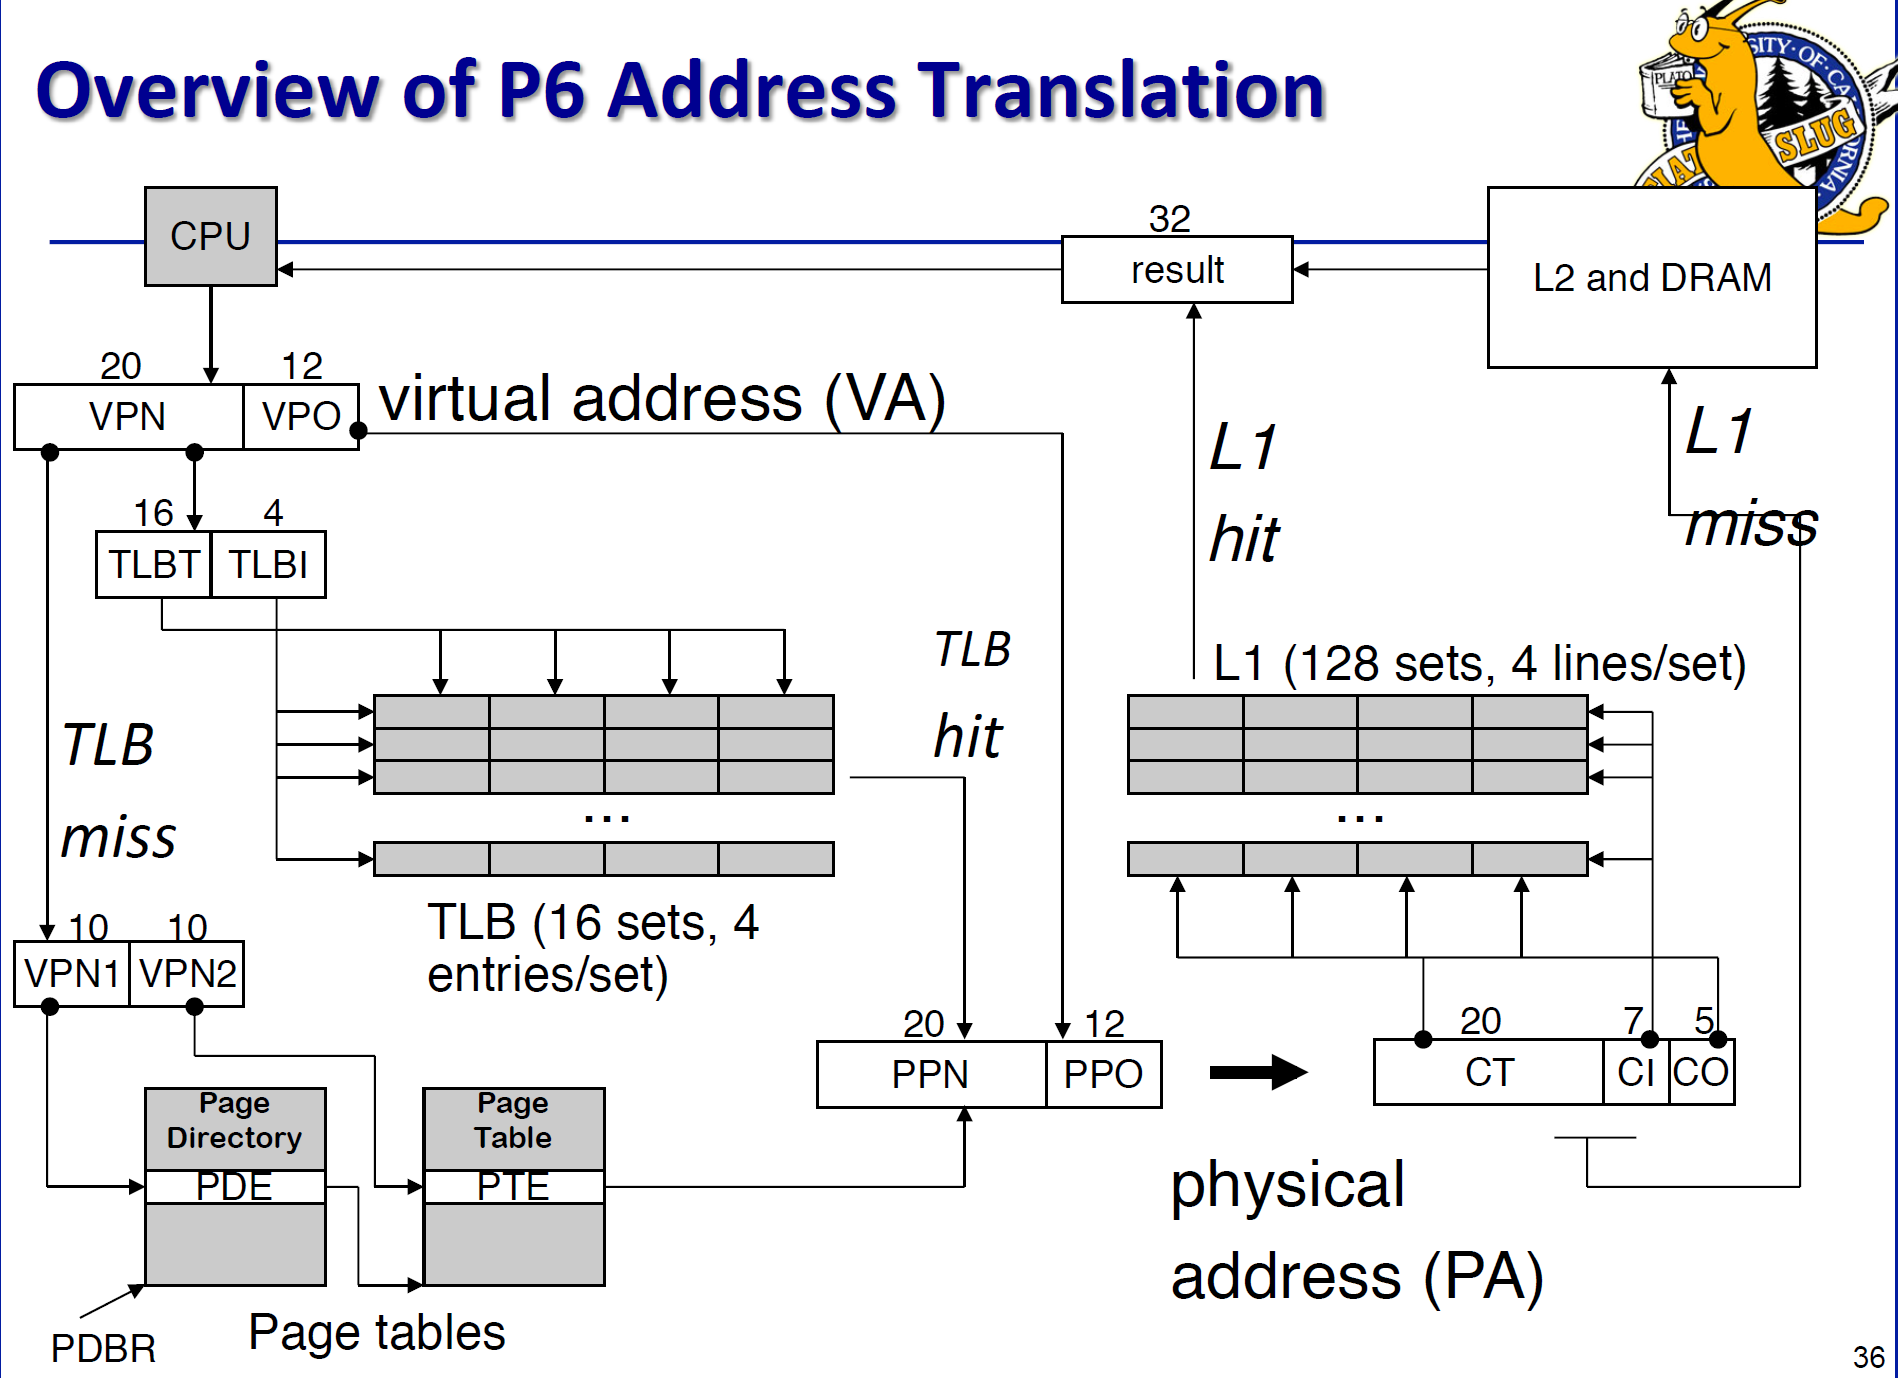
\includegraphics[scale=0.25]{virtual_address_translation.png}

\subsubsection*{I/O} I/O is measured by \code{throughput} (amount of data/time) and \code{latency} (response time to a single I/O operation). Common approach to I/O is use memory mapping. Devices separated into `block devices' and `stream devices'. Use \code{lseek(fp, offset, reference)}, \code{read(fp, buf, nbytes)}, \code{write(fp, buf, nbytes)}. Stream devices don't use addressing. Device drivers are low-level code to hide the interface. Hard drive accesses:
\begin{itemize}
    \item[] Queue delay if other requests pending
    \item[] Seek: move the heads (time given)
    \item[] Rotational latency (\(\tfrac{1}{2} / \) rotational speed)
    \item[] Data transfer (given)
    \item[] Controller overheads (given)
\end{itemize}
A bus is a shared communication link between devices with wires all connected in parallel. Can be synchronous (uses a clock) or not. Can increase transmission bandwidth using separate control/data lines, wider lines, block transfers. An initiator acquires the bus (may require arbiter), starts the transaction, specifies command, specifies address, specifies outbound data for write. Target responds to the action with data as necessary. Processory-memory bus (or processor-processor) is short, high-speed, designed to match memory system. I/O bus is usually long and slow.

\subsubsection*{PCI} 
\begin{itemize}
    \item[] \code{CLK} clock cycle
    \item[] \code{FRAME} is asserted by the device controlling the bus
    \item[] \code{AD} is the address of the target device and then holds responding data
    \item[] \code{C/BE} is the command, then the ID of the byte needed
    \item[] \code{IRDY} says the initiator is ready to receive data
    \item[] \code{TRDY} says the target is ready to transmit data
    \item[] \code{DEVSEL} says the target is connected
\end{itemize}

\subsubsection*{DMA} Direct Memory Access is a custom engine for data interface. Uses custom registers \code{from}, \code{to}, and \code{length}. Also has registers for status and control. Typically notifies processor operation is complete via interrupt. DMA engine will typically chain multiple operations such that \(\leq 1\) page is loaded at a time. DMA will use a \code{TLB} with virtual addresses.

\subsubsection*{Vectors} Implement data-level parallelism using vector instructions. Operate on vector registers. Perform single operations on multiple data elements. Amortizes instruction cost. Vector ALUs will be run in parallel in order to increase bandwidth. Domain specific hardware implements convolution engine to perform specific set of calculations really quickly. Uses a DMA to load/store data. 

\subsubsection*{FPGA} Field-programmable Gate Array is a 2-dimensional array of reconfigurable logic elements which implements Look-up tables, flip-flops, adders, Block RAM, and DSP blocks. Uses switch programmable interconnect to connect between array elements. Has I/O interface at chip boundary. 

\subsubsection*{Multicore:} Use shared memory accessed through loads/stores. Synchronization through atomic instructions \code{lr.w} and \code{st.w} which provide locking information. Multithreading executes more threads than cores. When 1 stalls, switch to another. Fine-grain MT switches threads each cycle. Coarse-grain MT switches threads on a long stall. Simultaneous MT uses multiple-issue dynamically scheduled pipeline hardware to exploit thread-level parallelism so it'll issue them as fast as it  can.

    \end{multicols}
\end{document}

